\section{Projektplan}
\subsection{Teoretisk bakgrund}
Skriv en teoretisk bakgrund som sammanfattar forskningsläget och beskriver det man redan vet och inte vet om ämnesområdet. Börja ganska allmänt med ett generellt problem som sätter in er undersökning i ett större sammanhang. Bli sedan mer specifika och inriktade mot er frågeställning. Källhänvisa till böcker, artiklar, hemsidor etc. i texten. Skriv den teoretiska bakgrunden utan underrubriker.

Längd: ½ -1 A4 (Times New Roman, 12 p, 1,5 radavstånd)

\subsection{Syfte}
Beskriv här syftet, alltså varför ni vill göra just i den här undersökningen, vad ni vill uppnå med resultaten eller hur resultaten kan bidra till förståelsen av det generella problem ni skrivit om i den teoretiska bakgrunden. Här skriver ni vad ni vill uppnå med ert gymnasiearbete. Ni kan till exempel börja med: Syftet med vårt gymnasiearbete är att beskriva/förklara/utvärdera/förstå … Beskriv också här kort hur ni planerar att uppnå syftet med arbetet. Ni kan till exempel skriva: I det här arbetet kommer vi att undersöka …
Längd: Ett par meningar

\subsection{Frågeställning och hypotes}
\textbf{Fråga:} ''Vad är den maximala hastigheten ett modelltåg i skala 1:40 kan uppnå vid en given kurvradie utan att spåra ur?''

\textbf{Hypotes:} Betrakta en järnvägsvagn i en vän3stersväng. Utgående från tågets referenssystem kommer kraftsituationen se ut som i \cref{fig:tåg_krafter_sväng}. Tyngdkraften ges som $F_g = mg$ där $m$ är tågets massa och tyngdaccelerationen $g\approx \SI{9.82}{\m\per\s\squared}$. Tågets centripetalacceleration $a_c$ ges som
\begin{equation}
        a_c = \frac{v^2}{r}
\end{equation}
 där $v$ är tågets hastighet tangent med svängen och $r$ är svängens radie. Därefter ges centripetalkraften $F_\mathrm{centripetal}$ genom att sätta $F = ma$ som
 \begin{equation}
    F_\mathrm{centripetal} = ma_c = \frac{mv^2}{r}.
 \end{equation}
 I tågets accelererande referenssystem kommer även centrifugalkraften $F_c$ finnas som
 \begin{equation}
    \vec F_c = -\vec F_\mathrm{centripetal}
 \end{equation}
 där sambandet $|\vec F_\mathrm{centripetal}| = |\vec F_c|$ gäller.

Både $F_c$ och $F_g$ utgör moment på fordonet kring en axel (se \cref{fig:tåg_krafter_sväng}). Dessa ges som
\begin{gather}
    M_g = F_g l_g \\
    M_c = F_c l_c.
\end{gather}
Man kan sedan intuitivt lista ut att tåget kommer välta när $M_g < M_c$  om positivt moment är utåt svängens riktning. Detta ger följande samband:
\begin{align*}
    M_g &< M_c \\
    F_g l_g &< F_c l_c \\
    mg l_g &< \frac{mv^2}{r} l_c \\
    g l_g &< \frac{v^2}{r} l_c \\
    g r \frac{l_g}{l_c} &< v^2 \\
    \left\{
        \begin{array}{l}
            v > \sqrt{g r \frac{l_g}{l_c}} \\
            v < -\sqrt{g r \frac{l_g}{l_c}}
        \end{array}
    \right.
\end{align*}

\begin{figure}[h!]
    \centering
    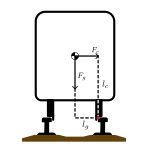
\includegraphics[width=0.33\textwidth]{fig/tåg_krafter.png}
    \caption{Kraftsituationen på en järnvägsvagn vid en vänstersväng där $F_g$ är tyngdkraften, $F_c$ är centrifugalkraften och $l_g$ respektive $l_c$ är deras momentarmar till rotationsaxeln A.}
    \label{fig:tåg_krafter_sväng}
\end{figure}

\subsection{Empirisk metod}
Skriv en kortfattad beskrivning av hur ni planerar att genomföra undersökningen och vilket material ni tänker att använda. Skriv också om, och i så fall hur, ni tänker använda kontroller och hur många upprepningar, replikat, ni kommer att ha. Källhänvisa om ni har hittat metoden i någon annans arbete. För att göra metodbeskrivningen tydlig, använd ord som: sedan, efter, därefter, slutligen, för det första, för det andra, för det tredje, etc. Skriv i löpande text och inte i en punktlista. Skriv om olika metoder under var sin underrubrik.
Längd: ½-1 A4
Analytisk metod
Beskriv hur ni planerar att analysera de data ni samlat in samt vilka beräkningar och formler ni då kommer att använda. Källhänvisa om ni har hittat analysmetoden i någon annans arbete.
Längd: Ett par stycken.

Materialen som kommer användas under undersökningen kommer vara: ett 3D printad tåg som väger ca 1,4 kg, en kamera som filmar i minst 240 FPS, ett stativ för att hålla kameran, rutat papper (med sidlängd 1 cm), 3D printade rälssegment.

Undersökningen kommer ske genom att det först väljs en viss radie. Därefter kommer tåget placeras på toppen av en backe med bestämd höjd. Målet med detta är att ge tåget en bestämd hastighet baserad på potentiel energi överförd till kenetisk energi. Sedan släpps tåget och resultaten från kameran och om den spårade ur eller ej skrivs ned. Om tåget inte har spårat ur kommer tåget placeras på en högre höjd och denna process repeteras tills tåget spårar ur. När tåget spårat ur välj en ny radie på kurvan och hela processen börjar om från början. När alla radier har testats kommer datan skrivas in i en graf där hastigheten och radien är grafens axlar.



\subsection{Tidsplan}
Här anger ni vad som ska göras, när det ska göras och vem som gör det.